\chapter{The S-GIVE Dataset}
\label{chap:s-give}
After GIVE 2.5 instalment presented in Chapter \ref{chap:give-challenge}, Prof. Kristina Striegnitz, Ph.D., one of the organizers of the GIVE Challenge, decided to collect a new dataset of spoken communication, called the S-GIVE Dataset. This chapter serves as an introduction to this dataset.

As a side note, \citet{striegnitz2012referring} report on a smaller German dataset, which is similar to the one I will be talking about. 

The S-GIVE dataset is different from previous GIVE Challenge experiments because the instructions were given by another person and were of a spoken form. In the following chapters, the term Instruction Giver (IG) will be used for the person giving instruction while the navigated person will be called Instruction Follower (IF). Also, let's assume the IG is a female and IF is a male.

The spoken form of instructions changes many aspects of the discourse. For one thing, the IG knows when the IF received her instruction, which is not true for the written instructions. That promotes faster feedback and allows interrupting during an instruction. However, in some cases, the spoken word tends to be less formal and grammatically correct. Moreover, interjections are very common, as are incomplete sentences. That makes the S-GIVE dataset complicated yet interesting to explore.

The data-collection started in July and finished in November of 2012. Through that period 21 interactions between two human subjects were recorded. Originally, 22 pairs participated, but one of the pair failed to finish the tasks and is excluded from the dataset. The subjects were asked to bring someone they know and they were financially compensated for the effort. 

The set-up for the experiment is shown in Figure \ref{fig:give-experiment-setup}. The role of IG, which is on the right in Figure \ref{fig:give-experiment-setup}, was essentially the role of the NLG system in the GIVE Challenge. She was able to see a map of the world, which was updated in real-time and she got information about all necessary steps to finish the task. In addition, she was able to see the other person's client screen. She communicated with the IF through a microphone and her goal was to navigate him through the world and make him finish the treasure-hunt.

\begin{figure}[!htbp]
  \centering
	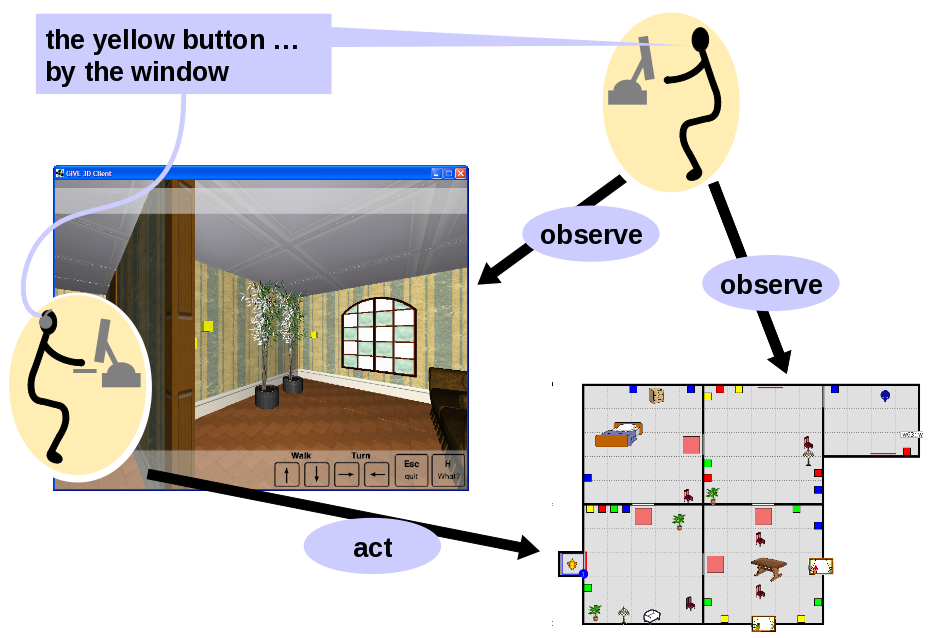
\includegraphics[width=0.7\textwidth]{Images/experiment-set-up}
	\caption{Experiment set-up of data collection}
	\label{fig:give-experiment-setup}
\end{figure}

The IF is on the left in Figure \ref{fig:give-experiment-setup}. He interacted with the client and moved the avatar around the world and was able to press buttons. He listened to the IG's instructions through a headset.

Each pair played one short tutorial world. After that they switched the roles of instruction giver and instruction follower. Following the tutorial was one ``normal'' world randomly chosen from two variants, marked world 1 and world 3 in the dataset. Maps of the worlds 1 and 3 are in Figures \ref{fig:dataset-world1} and \ref{fig:dataset-world3} respectively. Finally they did a difficult version of the other variant (if they started with world 1 the difficult version was for world 3 and vice versa). The difficult versions are marked 1-d and 3-d in the dataset. A difficult version of the world had an increased number of distracting buttons and landmarks compared to the ``normal'' version, as can be seen in the map of world 1-d in figure \ref{fig:dataset-world1d}. If not not stated otherwise, the short tutorial worlds are normally excluded from the analysis.

\begin{figure}[!htbp]
  \centering
	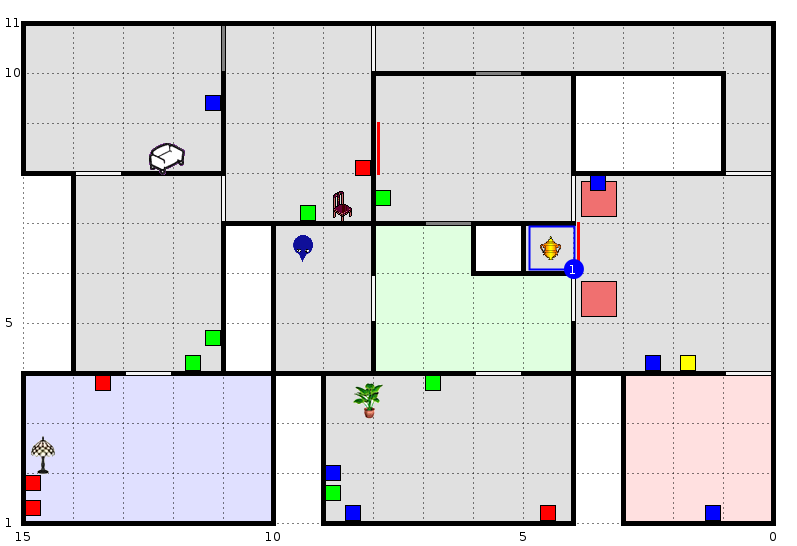
\includegraphics[width=0.7\textwidth]{Images/dataset-world1}
	\caption{Map of the world 1 - normal version.}
	\label{fig:dataset-world1}
\end{figure}

\begin{figure}[!htbp]
  \centering
	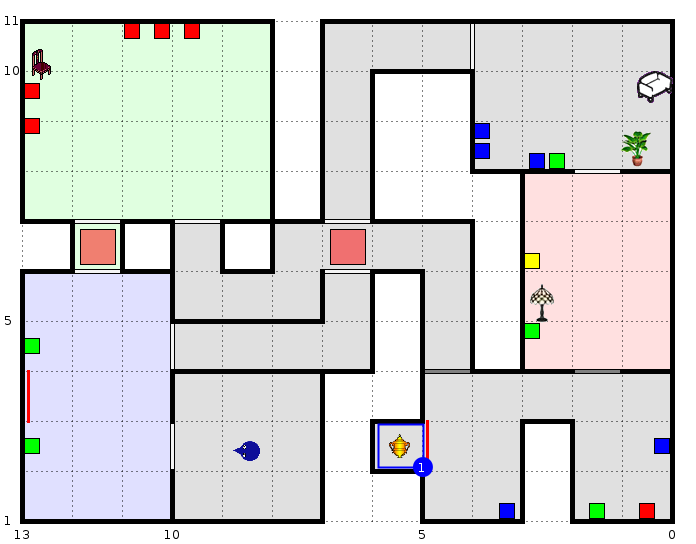
\includegraphics[width=0.7\textwidth]{Images/dataset-world3}
	\caption{Map of the world 3 - normal version.}
	\label{fig:dataset-world3}
\end{figure}

\begin{figure}[!htbp]
  \centering
	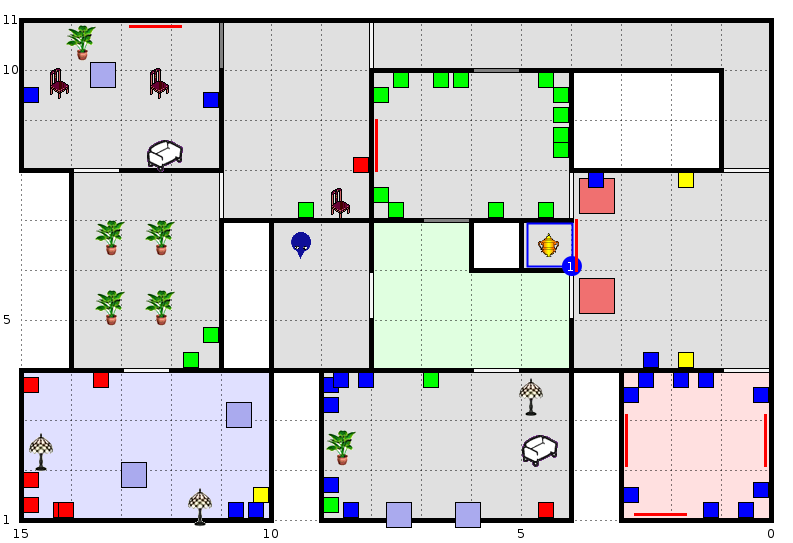
\includegraphics[width=0.7\textwidth]{Images/dataset-world1d}
	\caption{Map of the world 1 - difficult version.}
	\label{fig:dataset-world1d}
\end{figure}

Similarly to the GIVE Challenge, after all 3 rounds subjects were asked to fill in a questionnaire. Its purpose was to get demographic and other relevant information on subjects. The questionnaire can be divided into three parts. The first part was only filled out by the IF and rated the IG and his instruction giving on a scale from 1 to 7. The complete list of the first part questions follows: 

\begin{enumerate}
\item
Overall, my partner gave me good instructions.
\item
Interacting with my partner wasn't annoying at all.
\item
My partner's instructions were clearly worded.
\item
When I had problems with the instructions, we solved them quickly.
\item
I enjoyed solving the task.
\item
I felt I could trust my partner's instructions.
\item
I really wanted to find that trophy.
\item
My partner immediately offered help when I was in trouble.
\item
I would recommend this experiment to a friend.
\item
My partner's instructions were not repetitive.
\end{enumerate}


The second part was filled by both the IF and the IG and was concerned with their navigation skills. To measure the ability to navigate in the world the Santa Barbara Sense of Direction (SBSOD) scores were used \citep{hegarty2002development}. Again the questions were on a scale from 1 to 7. Note that some of the question in the following list are of positive nature (higher rating equals better navigation skill) while other are of negative nature, therefore these scores had to be normalized.

\begin{enumerate}
\item
I am very good at giving directions.
\item
I have a poor memory for where I left things.
\item
I am very good at judging distances.
\item
My "sense of direction" is very good.
I tend to think of my environment in terms of cardinal directions (N, S, E, W).
\item
I very easily get lost in a new city.
\item
I enjoy reading maps.
\item
I have trouble understanding directions.
\item
I am very good at reading maps.
\item
I don't remember routes very well while riding as a passenger in a car.
\item
I don't enjoy giving directions.
\item
It's not important to me to know where I am.
\item
I usually let someone else do the navigational planning for long trips.
\item
I can usually remember a new route after I have travelled it only once.
\item
I don't have a very good "mental map" of my environment.
\end{enumerate}


Finally, the last part of the questionnaire was of a demographic character. We can see questions about age, gender, language and computer expertise, 3D games experience and knowledge of the partner in the following list.

\begin{enumerate}
\item
What is your age?
\item
Are you male of female?
\item
What is your profession / major / favorite subject in school?
\item
How would you rate your computer expertise?
\item
How familiar are you with 3D computer games?
\item
How many hours per week to you play 3D computer games?
\item
Was there a time in your life when you played more 3D computer games? If so, how many hours did you play then?
\item
What languages do you speak? Please indicate how well you speak each on a scale from 1-5, where 5 is your native language.
\item
Did you already know the second participant?
\item
How well do you know the second participant?
\item
Have you worked collaboratively with the second participant before? (For example, when doing homework or preparing a class presentation?)
\item
Have you played 3D computer games with the second participant before?
\end{enumerate}

Many of these questions are explored in the next chapter as potential factors influencing the task performance. 

As was mentioned in Chapter \ref{chap:give-challenge}, the entire session is logged to a database. The player's position, orientation and all visible objects are logged at a fixed rate, approximately every 200 ms. Moreover, other information such as buttons presses or the end of the session are also stored in the logs. Because the worlds are static, distances and angles between the IF and other game objects are easily computed from these logs.

Apart from the logs, there are of course sound files of the IG giving directions. These were transcribed and together with some information from the logs transformed into ELAN files. ELAN is an annotation software \citep{sloetjes2008annotation}. The term \textit{automatic annotations} will be used for the ELAN files created from the logs and transcribed audio in the following text (however note that transcribing audio was done manually). 

These automatic annotations served as a base for creating manual annotations. Manual annotations are primarily concerned with referring expressions and also stored in ELAN format. Most referring expressions in GIVE aim to locate a button, which needs to be pressed. The button, which is a goal of a referring expression, will be called the target button in the following text. Which button is the target button of a reference is one of the layers in the manual annotations. Another layer of the annotations is some basic categorization of the references, whether it is a reference to a single button, to a group of button, to a landmark and so on. The third layer looks deeper into the contents of the reference. It notes whether the reference contains for example the color of a button, whether distractors or landmarks are part of the reference or whether the reference explicitly points out that the button was already pressed before.

The previously mentioned logs, automatic annotations and manual annotations together form the dataset this chapter is dealing with.

An example of an interaction between an IF and an IG is in the following text. Spatial information is transcribed in parentheses for the sake of clearness.

\begin{verse}
(IF enters a room)\\
IG: Go towards the red buttons.\\
(IF turns right and start walking, but he turns too much)\\
IG: No the ones next to the lamp...\\
(IF corrects his direction)\\
IG: Yeah that lamp. On the right.\\
(IF is facing three buttons.)\\
IG: Press the button on the wall you are looking at, that's far from the lamp and on the left. \\
(IF goes towards the correct button and stops close to him)\\
IG: Press it.\\
\end{verse}

After introducing the S-GIVE dataset, the next chapter will contain my analysis of it and machine learning attempts on it.




